%!TEX root =  cpt-rl-icml.tex

For a real-valued random variable $X$, we introduce a ``CPT-functional'' that replaces the traditional expectation operator. 
%Subsequently, we specialize $X$ to be the return of stochastic shortest path problem. 
%\subsection{General definition}
%\label{sec:cptdef}
The functional, denoted by $\C$, will be 
indexed by
$u=(u^+,u^-)$ and $w=(w^+,w^-)$. 
As illustrated in Figure \ref{fig:u}, $u^+,u^-:\R\rightarrow \R_+$ are continuous,
with $u^+(x)=0$ when $x\le 0$ and increasing otherwise, and with $u^-(x)=0$ when $x\ge 0$ and decreasing otherwise.
The functions $w^+,w^-:[0,1] \rightarrow [0,1]$, as shown in Figure \ref{fig:w}, are continuous, non-decreasing and  satisfy $w^+(0)=w^-(0)=0$ and $w^+(1)=w^-(1)=1$.
%(see assumptions (A1)-(A2) in Section \ref{sec:cpt-sampling} for precise requirements on $u$ and $w$).
The CPT-functional indexed by $u$ and $w$ is defined as 
\begin{align}
\C_{u,w}(X) &= \intinfinity w^+\left(\Prob{u^+(X)>z}\right) dz\nonumber \\
&\quad - \intinfinity w^-\left(\Prob{u^-(X)>z}\right) dz\,. \label{eq:cpt-general}
\end{align}
For notational convenience, when $u,w$ are fixed, we drop the dependence on them and use $\C(X)$ to denote the CPT-value of $X$. 

Consider the case when $w^+,w^-$ are identity functions,  
$u^+(x)=x$ for $x\ge0$ and $0$ otherwise and $u^-(x)=-x$ for $x\le0$ and $0$ otherwise. Then,  letting $(a)^+ = \max(a,0)$, $(a)^- = \max(-a,0)$, we have 
$\C(X) = \intinfinity \Prob{X>z} dz -  \intinfinity \Prob{-X>z} dz = \EE{ (X)^+ } - \EE{ (X)^- }$, showing the connection to expectations.
%\cref{fig:u} shows an example of the utility functions $u= (u^+,u^-)$ and how they relate to each other, while \cref{fig:w} shows an example of a typical weight function.
 \begin{figure}[t]
   \centering
\tabl{c}{
%\includegraphics[width=3.8in]{utility.png}}
   \scalebox{0.5}{\begin{tikzpicture}
   \begin{axis}[width=13cm,height=6.5cm,legend pos=south east,
          %  grid = major,         
            axis lines=middle,
           % grid style={dashed, gray!30},
            xmin=-5,     % start the diagram at this x-coordinate
            xmax=5,    % end   the diagram at this x-coordinate
            ymin=-4,     % start the diagram at this y-coordinate
            ymax=4,   % end   the diagram at this y-coordinate
           % axis background/.style={fill=white},
            ylabel={\large\bf Utility},
            xlabel={\large\bf Gains},
            x label style={at={(axis cs:4.7,-0.8)}},
            y label style={at={(axis cs:-0.8,4.8)}},
            xticklabels=\empty,
            yticklabels=\empty
            ]
           \addplot[name path=cptplus,domain=0:5, green!35!black, very thick,smooth] 
              {pow(abs(x),0.8)}; 
            \addplot[name path=cptminus,domain=-5:0, red!35!black,very thick,smooth] 
              {-2*pow(abs(x),0.7)}; 
               \addplot[domain=-5:5, blue, thick]           {x}; 
               
               \path[name path=diagplus] (axis cs:0,0) -- (axis cs:5,5);
 			  \path[name path=diagminus] (axis cs:-5,-5) -- (axis cs:0,0);
                \path[name path=xaxisplus] (axis cs:0,0) -- (axis cs:5,0);
                 \path[name path=xaxisminus] (axis cs:-5,0) -- (axis cs:0,0);
                 \path[name path=yaxisplus] (axis cs:0,0) -- (axis cs:0,5);
                 \path[name path=yaxisminus] (axis cs:0,-5) -- (axis cs:0,0);
 
 \addplot [orange!40]  fill between[of= diagminus and yaxisminus];
 \addplot [cyan!20]  fill between[of= diagplus and xaxisplus];
 
 \node at (axis cs:  -3.7,-0.45) {\large\bf Losses};
 \node at (axis cs:  4,2.5) {\large $\bm{u^+}$};
 \node at (axis cs:  -1,-3) {\large $\bm{-u^-}$};
% \node at (axis cs:  2.5,-2.5) {\large\bf Baseline};
%\draw[-{>[scale=2.5,
%          length=5,
%          width=3]},thick] (axis cs:2,-2) -- (axis cs:0,0);
   \end{axis}
   \end{tikzpicture}}}\\[1ex]
\caption{An example of a utility function. A reference point on the $x$ axis serves as the point of separating gains and losses.
For losses, the disutility $-u^-$ is typically convex and for gains, the utility $u^+$ is typically concave; 
both functions are non-decreasing and take the value of zero at the reference point.}
\label{fig:u}
\end{figure}



In the definition, $u^+, u^-$ are utility functions corresponding to gains ($X \ge 0$) and losses ($X \le 0$), respectively,
where zero is chosen as an arbitrary ``reference point'' to separate gains and losses.
Handling losses and gains separately is a salient feature of CPT, and this addresses the tendency of humans to play safe with gains and take risks with losses. % - see Fig \ref{fig:u}. 
To illustrate this tendency, 
consider a scenario where one can either earn \$$500$ with probability (w.p.) $1$ or earn \$$1000$ w.p. $0.5$ and nothing otherwise. 
The human tendency is to choose the former option of a certain gain. 
If we flip the situation, i.e., a certain loss of \$$500$ or a loss of \$$1000$ w.p. $0.5$, 
then humans choose the latter option.  
This distinction of playing safe with gains and taking risks with losses is captured by a concave gain-utility
$u^+$ and a convex disutility $-u^-$, as illustrated in \cref{fig:u}.
%In contrast, the traditional value function makes no such distinction between gains and losses.  

\begin{figure}[h]
\centering
\tabl{c}{
%\includegraphics[width=8cm]{results/Probability_weighting_function.jpg}
  \scalebox{0.65}{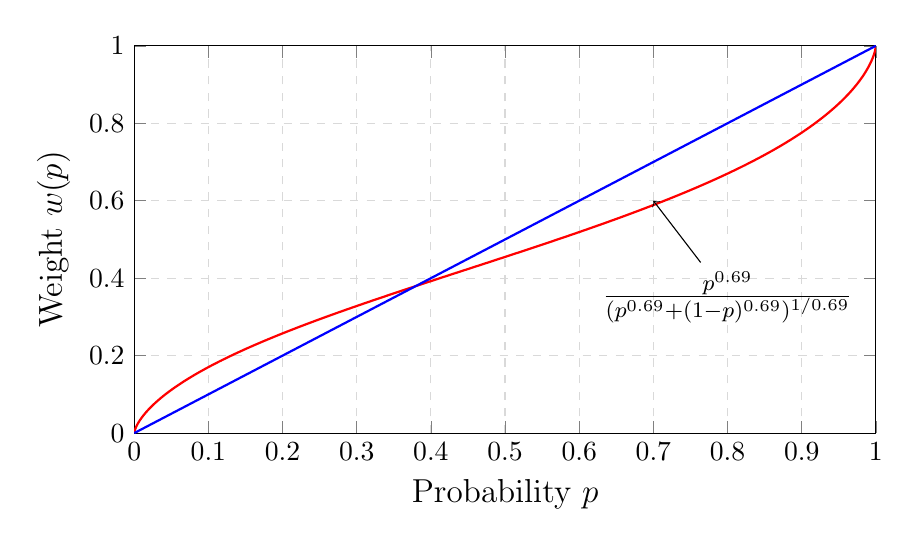
\begin{tikzpicture}
  \begin{axis}[width=11cm,height=6.5cm,legend pos=south east,
           grid = major,
           grid style={dashed, gray!30},
           xmin=0,     % start the diagram at this x-coordinate
           xmax=1,    % end   the diagram at this x-coordinate
           ymin=0,     % start the diagram at this y-coordinate
           ymax=1,   % end   the diagram at this y-coordinate
           axis background/.style={fill=white},
           ylabel={\large Weight $\bm{w(p)}$},
           xlabel={\large Probability $\bm{p}$}
           ]
          \addplot[domain=0:1, red, thick,smooth,samples=1500] 
             {pow(x,0.69)/pow((pow(x,0.69) + pow(1-x,0.69)),1.44)}; 
             \node at (axis cs:  0.8,0.35) (a1) {\large $\bm{\frac{p^{0.69}}{(p^{0.69}+ (1-p)^{0.69})^{1/0.69}}}$};           
             \draw[->] (a1) -- (axis cs:  0.7,0.6);
                 \addplot[domain=0:1, blue, thick]           {x};                      
  \end{axis}
  \end{tikzpicture}}\\[1ex]
}
\caption{An example of a weight function.
A typical CPT weight function inflates small, and deflates large probabilities, capturing the 
tendency of humans doing the same when faced with decisions of uncertain outcomes.
}
\label{fig:w}
\end{figure}

The functions $w^+, w^-$, called the weight functions, capture the idea that humans deflate high-probabilities and inflate low-probabilities.
For example, humans usually choose a stock that gives a large reward, e.g., 
one million dollars w.p. $1/10^6$, over one that gives \$$1$ w.p. $1$ and the reverse when signs are flipped. 
Thus the value seen by a human subject is nonlinear in the underlying probabilities -- an observation backed by strong empirical evidence \cite{tversky1992advances,Barberis:2012vs}.  
%In contrast, the expected utility is linear in the underlying probabilities. 
In \cite{tversky1992advances}, the authors recommend $w(p) = \frac{p^{\eta}}{{(p^{\eta}+ (1-p)^{\eta})}^{1/\eta}}$, while in \cite{prelec1998probability}, the author recommends $w(p) = \exp(-(-\ln p)^\eta)$, with $0 < \eta <1$. In both cases, the weight function has an inverted-s shape.
% which is seen to be a good fit from empirical tests on human subjects - see \cite{conlisk1989three}, \cite{camerer1989experimental}, \cite{camerer1992recent}, \cite{harless1992predictions}, \cite{sopher1993test}, \cite{camerer1994violations}, \cite{gonzalez1999shape}, \cite{abdellaoui2000parameter}.  
\if0
Weight functions can explain nonlinear probability distortions, as illustrated by the following example: \\
\textit{\textbf{[Stock 1]}} This investment results in a gain of \$$10$ with probability (w.p.) $0.1$ and a loss of \$$500$ w.p. $0.9$. The expected return is \$$-449$, but this does not necessarily imply that ``human'' investors' evaluation of the stock is \$$-449$. Instead, it is very likely that the humans evaluate it to a higher value, e.g. \$$-398$ ($=$ gain w.p. $0.2$ and loss w.p. $0.8$).\footnote{See Table 3 in \cite{tversky1992advances} to know why such a human evaluation is likely.}\\
\textit{\textbf{[Stock 2]}} loss of \$$10$ w.p. $0.9$, gain \$$500$ w.p. $0.1$. Expected return: \$$41$; Human evaluation: \$$92$ ($=$ loss w.p. $0.8$).\\
\textit{\textbf{[Stock 3]}} loss of \$$10$ w.p. 0.1, gain \$$500$ w.p. $0.9$. Expected return: \$$449$; Human evaluation: \$$398$ ($=$ loss w.p. $0.2$). 
\fi



%A few remarks are in order.
\begin{remark}\textit{(RL application)}
%The CPT-value, as defined in \eqref{eq:cpt-general}, has several applications in RL. In general, 
For any RL problem setting, one can define the return for a given policy and then apply a CPT-functional on the return. For instance, with a fixed policy, the random variable (r.v.) $X$ could be the total reward in a stochastic shortest path problem or the infinite horizon cumulative reward in a discounted MDP.
 %- See Appendix \ref{sec:cpt-ssp} for one such application. 
\end{remark}


%\subsection{Application: Stochastic Shortest Path}
%We consider a stochastic shortest path (SSP) problem with states $\S=\{0,\ldots,\L\}$, where $0$ is a special reward-free absorbing state.  A randomized policy $\pi$ is a function that maps any state $s\in \S$ onto a probability distribution over the actions $\A(s)$ in state $s$. As is standard in policy gradient algorithms, we parameterize $\pi$ and assume it is continuously differentiable in its parameter $\theta \in \R^d$.  
%An \textit{episode} is a simulated sample path using policy $\theta$ that starts in state $x^0\in \S$, visits $\{x_1,\ldots, x_{\tau-1}\}$ before ending in the absorbing state $0$, where $\tau$ is the first passage time to state $0$.
%Let $D^\theta(s^0)$ be a random variable (r.v) that denote the total reward from an episode, defined by
%$$ D^\theta(s^0) = \sum\limits_{m=0}^{\tau-1} r(s_m,a_m), $$
%where the actions $a_m$ are chosen using policy $\theta$ and $r(s_m, a_m)$ is the single-stage reward in state $s_m\in \S$ when action $a_m \in \A(s_m)$ is chosen. 
%
%Instead of the traditional RL objective for an SSP of maximizing the expected value $\E (D^\theta(s^0))$, 
%we adopt the CPT approach and aim to solve the following problem: 
%$$ \max_{\theta \in \Theta} \C(D^\theta(s^0)),$$
%where $\Theta$ is the set of admissible policies that are \textit{proper}\footnote{A policy $\theta$ is proper if $0$ is recurrent and all other states are transient for the Markov chain underlying $\theta$. It is standard to assume that policies are proper in an SSP setting - cf. \cite{bertsekas1995dynamic}.} and the CPT-value function $\C(D^\theta(s^0))$ is defined as
%\begin{align}
%\C(D^\theta(s^0))& = \intinfinity w^+(P(u^+(D^\theta(s^0)))>z) dz \nonumber
%\\&- \intinfinity w^-(P(u^-(D^\theta(s^0)))>z) dz. \label{eq:cpt-mdp}
%\end{align}

\begin{remark}\textit{(Generalization)}
As noted earlier, the CPT-value is a generalization of mathematical expectation. 
It is also possible to obtain \eqref{eq:cpt-general} to coincide with other risk measures, for e.g. value at risk (VaR) and conditional value at risk (CVaR), by appropriate choice of weight functions.
\end{remark}

%\begin{remark}\textit{(Sensitivity)}
%\todoc{I think this is really hard to defend.
%Since the derivative of the weight function at zero is very high (even zero),
%the CPT value is hugely sensitive (even more so than the expected value) to error
%in low probabilities. We should remove this remark.
%}
%Traditional EU-based approaches are sensitive to modeling errors as illustrated in the following example: 
%Suppose stock $\cal{A}$ gains \$$10000$ w.p $0.001$ and loses nothing w.p. $0.999$, while stock $\cal B$ surely gains $11$. With the classic value function objective, it is optimal to invest in stock $\cal B$ as it returns $11$,  while $\cal A$ returns $10$ in expectation (assuming utility function to be the identity map). Now, if the gain probability for stock $\cal A$ was $0.002$, then it is no longer optimal to invest in stock $\cal B$ and investing in stock $A$ is optimal.
%Notice that a very slight change in the underlying probabilities resulted in a big difference in the investment strategy and a similar observation carries over to a multi-stage scenario (see the house buying example in the numerical experiments section). 
 %%A randomized policy that $50$\% in stock $\cal A$ and the rest in a risk-free asset is less sensitive to the error in under-estimating the loss probability. 
%
%Using CPT makes sense because it inflates low probabilities and thus can account for modeling errors, especially considering that model information is unavailable in practice.
%Note also that in MDPs with expected utility objective, there exists a deterministic policy that is optimal. However, with CPT-value objective, the optimal policy is \textit{not necessarily} deterministic - See also the organ transplant example on pp. 75-81 of \cite{lin2013stochastic}. 
%\end{remark}

